\section{System Architecture}

A huge end-goal of ours is to have a public system where participating users' phones transmit sensor information to a central database through a REST-based web service. The service stores this information in the database and another data processing system. Other users who are not contributing information can connect to our system to access other related services, like a choropleth map of the sensor data; BAC prediction data in our case, but the system would not be limited to it. The particular protocols and setup used should be designed to protect the privacy of the sensor data contributors.

\begin{figure}
	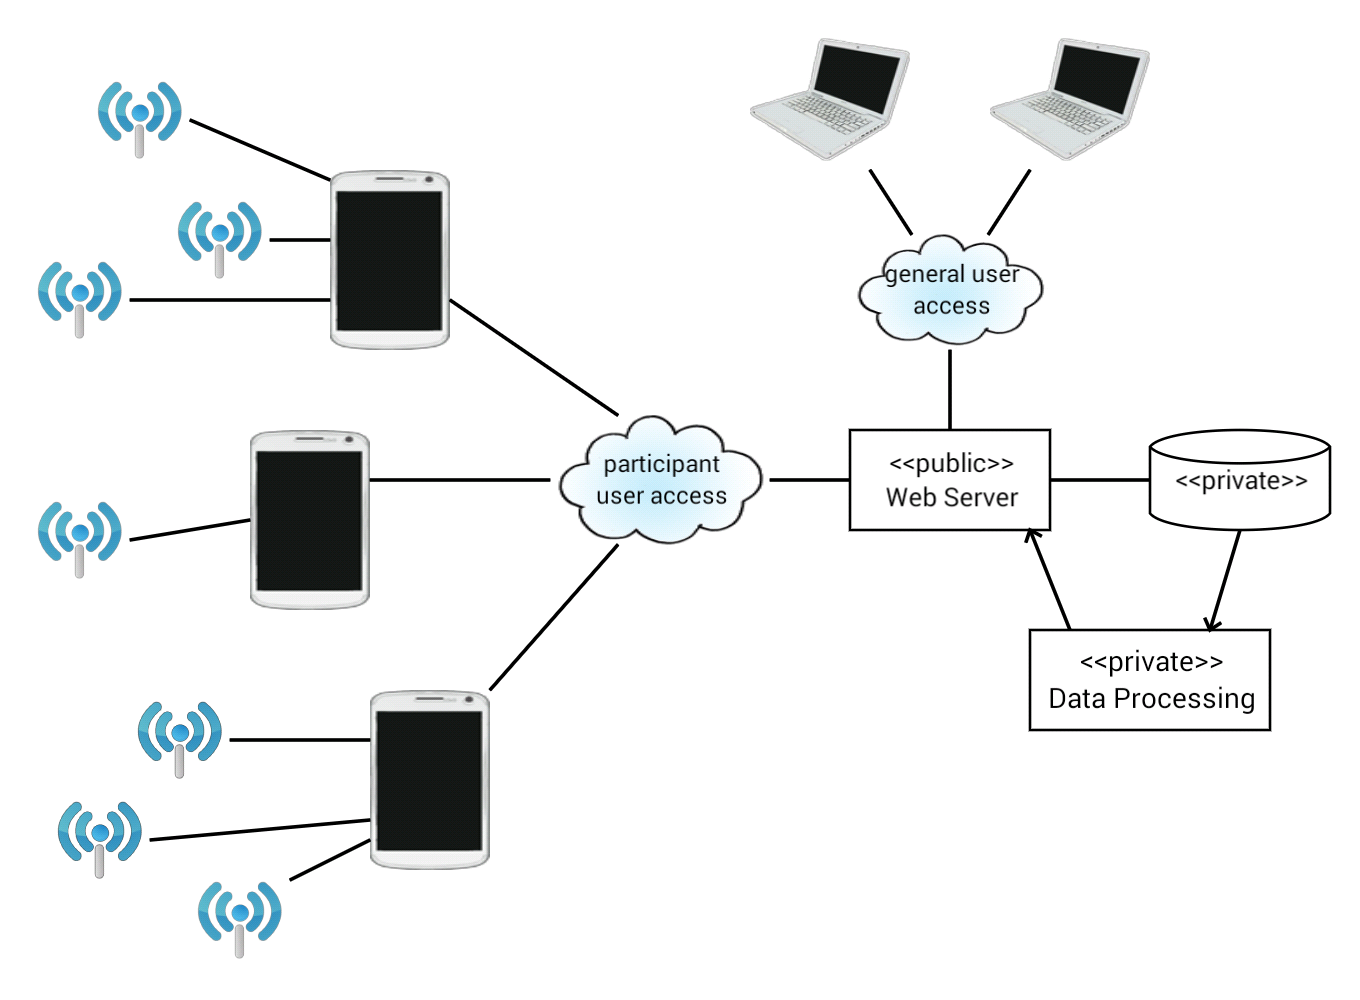
\includegraphics[width=1.0\textwidth]{figs/system}
	\caption{Example general system for large-scale sensor data collection}
	\label{fig:system}
\end{figure}

\subsection{Smartphone Sensor Gateway}

Each of the smartphones in this system are behaving as a type of sensor gateway. In order to collect our data, we built such a system on the Android platform. Though we used primarily a Microsoft Band, our system allows the easy addition of any sensor that can be connected to from the Android smartphone. In Figure \ref{fig:gateway}, we show an overview of the classes used in this system.

\begin{figure}
	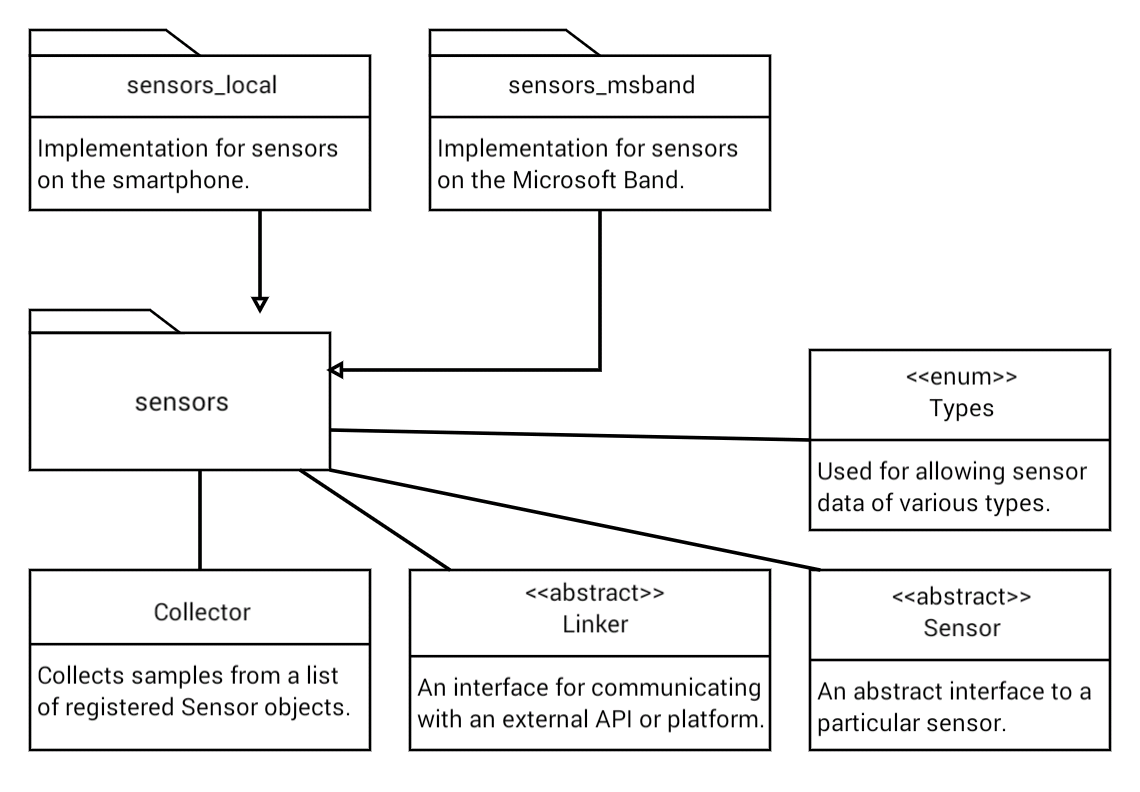
\includegraphics[width=1.0\textwidth]{figs/gateway}
	\caption{Gateway implementation for our data collection application}
	\label{fig:gateway}
\end{figure}
